%%%%%%%%%%%%%%%%%%%%%%%%%%%%%%%%%%%%%%%%%%%%%%%%%%%%%%%%%%%%%%%%%%%%%%%%
%    INSTITUTE OF PHYSICS PUBLISHING                                   %
%                                                                      %
%   `Preparing an article for publication in an Institute of Physics   %
%    Publishing journal using LaTeX'                                   %
%                                                                      %
%    LaTeX source code `ioplau2e.tex' used to generate `author         %
%    guidelines', the documentation explaining and demonstrating use   %
%    of the Institute of Physics Publishing LaTeX preprint files       %
%    `iopart.cls, iopart12.clo and iopart10.clo'.                      %
%                                                                      %
%    `ioplau2e.tex' itself uses LaTeX with `iopart.cls'                %
%                                                                      %
%%%%%%%%%%%%%%%%%%%%%%%%%%%%%%%%%%
%
%
% First we have a character check
%
% ! exclamation mark    " double quote  
% # hash                ` opening quote (grave)
% & ampersand           ' closing quote (acute)
% $ dollar              % percent       
% ( open parenthesis    ) close paren.  
% - hyphen              = equals sign
% | vertical bar        ~ tilde         
% @ at sign             _ underscore
% { open curly brace    } close curly   
% [ open square         ] close square bracket
% + plus sign           ; semi-colon    
% * asterisk            : colon
% < open angle bracket  > close angle   
% , comma               . full stop
% ? question mark       / forward slash 
% \ backslash           ^ circumflex
%
% ABCDEFGHIJKLMNOPQRSTUVWXYZ 
% abcdefghijklmnopqrstuvwxyz 
% 1234567890
%
%%%%%%%%%%%%%%%%%%%%%%%%%%%%%%%%%%%%%%%%%%%%%%%%%%%%%%%%%%%%%%%%%%%
%
\documentclass[12pt]{iopart}
\newcommand{\gguide}{{\it Preparing graphics for IOP Publishing journals}}
%Uncomment next line if AMS fonts required
\usepackage{iopams}  
\usepackage{graphicx}
%\usepackage{amsmath,amssymb}
\begin{document}

\title[]{Leveraging local continuity of connected measurements for dimensionality reduction and separation of backround, signal, and noise.... }

\author{}

%%\address{IOP Publishing, Temple Circus, Temple Way, Bristol BS1 6HG, UK}
%\ead{submissions@iop.org}
%\vspace{10pt}
%\begin{indented}
%%\item[]August 2017
%\end{indented}

%\begin{abstract}
%This document describes the  preparation of an article using \LaTeXe\ and 
%\verb"iopart.cls" (the IOP Publishing \LaTeXe\ preprint class file).
%This class file is designed to help 
%authors produce preprints in a form suitable for submission to any of the
%journals listed in table~\ref{jlab1} on the next page.  You are not obliged to use this class file---we accept
%submissions using all common \LaTeX\ class and style files.  The \verb"iopart.cls"
%class file is supplied merely as a convenience for those authors who find it useful.
%This document gives both general advice that applies whatever class file you use, and specific advice
%that applies if you choose to use \verb"iopart.cls".
%
%We also accept submissions in Word format.  See elsewhere on this site for guidelines on Word submissions.
%
%If you have any queries about this document or any aspect of preparing your article for submission please contact us at the e-mail address given above.
%\end{abstract}

%
% Uncomment for keywords
%\vspace{2pc}
%\noindent{\it Keywords}: XXXXXX, YYYYYYYY, ZZZZZZZZZ
%
% Uncomment for Submitted to journal title message
%\submitto{\JPA}
%
% Uncomment if a separate title page is required
%\maketitle
% 
% For two-column output uncomment the next line and choose [10pt] rather than [12pt] in the \documentclass declaration
%\ioptwocol
%



\section{Introduction}
Experiments undertaken at synchrotron and XFEL light sources can generate large volumes of data that are rich in information but plagued by noise and artifacts. There is often much continuity between successive measurements: when collecting a progression of diffraction patterns or spectra over a continuous range of physical states, the standard practice is to capture many intermediate states of the corresponding evolution of the signal. Furthermore many methods--such as powder diffraction and serial crystallography--require repeated measurements of the same system to accumulate sufficient statistics or orientational averaging. 

%Define ordered and connected

For these two reasons large spectroscopic or diffraction datasets generated in typical experiments at third- or fourth-generation light sources are likely to contain sequences of measurements with smooth variation with respect to the underlying physical information. Equivalently, we say that such a dataset can be assembled into a high-dimensional array where the underlying signal is both \emph{smooth} and \emph{connected}. More explicitly, any such dataset can be represented as the tensor

\begin{equation}
X_{i_1i_2...i_Nq}
\end{equation}

for which each distinct sequence of values for the indices $i_1, i_2,...
i_N$ corresponds to a single spectrum or diffraction pattern, $q$
indexes momentum transfer or energy in the case of XRD or spectroscopy,
respectively, and each of the indices $i_n, n \in \{1, 2, ... N\}$
corresponds to an ordering dimension along which direction the
underlying signal's variation is smooth. The dimensionality of the
dataset is thus simply one higher than $N$, the number of ordinal
attributes.


This connectedness describes both the signal and any smoothly-varying
background, while other contributions to the measured X-ray
intensity--such as shot noise, one-off artifacts, and stochastic
variations across different portions of the sample--are uncorrelated or
at least substantially stochastic. (note: high-frequency variation is a
more accurate description here, uncorrelated is a limiting case but it
simplifies the interpretation).

In this paper, we take two examples of XRD datasets--one temperature
study of xxxx material and one combinatorial study of the CoNiTi
ternary system--to demonstrate the separation of connected data into
a physically 'meaningful' component and a component that comprises
noise and artifacts. At the most basic level, we see that the signal
is readily separated into two components: $X = \hat{X} + \eta$, where
$\hat{X}$ is a slow-varying signal and $\eta$ is a fast-varying noise
contribution. The approach depends only on the minimal assumption of
connectedness and so should be applicable, with minor tuning, to any
dataset.

%use  connectedness of measurements to separate a collection of spectral or diffraction
%
%In this paper we consider ways in which the redundancy of datasets connected by 
%
%This redundancy, we argue, creates an opportunity to use the mutual information accross different measurements to make.... information... robust or whaterver.... 
%
%Rich in information, plagued by noise and artifacts. 
%
%IN the paper, we want to show how we can leverage the connectedness of the measurements ... yada yadaa minimal assumptions, separate useful information from these large datasets.
%
%1. LS collect connected datasets
%2. rich in information but also artifacts and noise (background, peak shifting artifact, noise)
%    2. a Introduce Yijin and Suchi's data
%3. leveraging connectedness, we can separate these datasets. -> expand into the body of the paper.
%    3. a Define connectedness, state assumptions. Good measurements oversample the measrement space. We can use this oversampling to help separate datasets into different components with minimal assumptions. Connect 
%(work on the title)

%## Introduction
%* aim for JSR? large facilities (synchrotron, XFEL) produce large connected datasets (cites). 
%* Neighborhood and continuity can be exploited in two ways: to estimate noise (in the absence of a noise model) and to extract features. 
%* Motivating applications: combi; any 'dense' dataset over a range of values for the key experimental parameter.
%* Motivating problem: peak shifting is difficult to model; naive similarity metrics are not robust to it. What's the most parsimonious way of grouping XRD patterns for structures that are the same up to lattice parameter distortions? We will show that continuity + neighborhood is sufficient.
%* Discuss, cite prior literature

\section{Methods}
\begin{figure}
  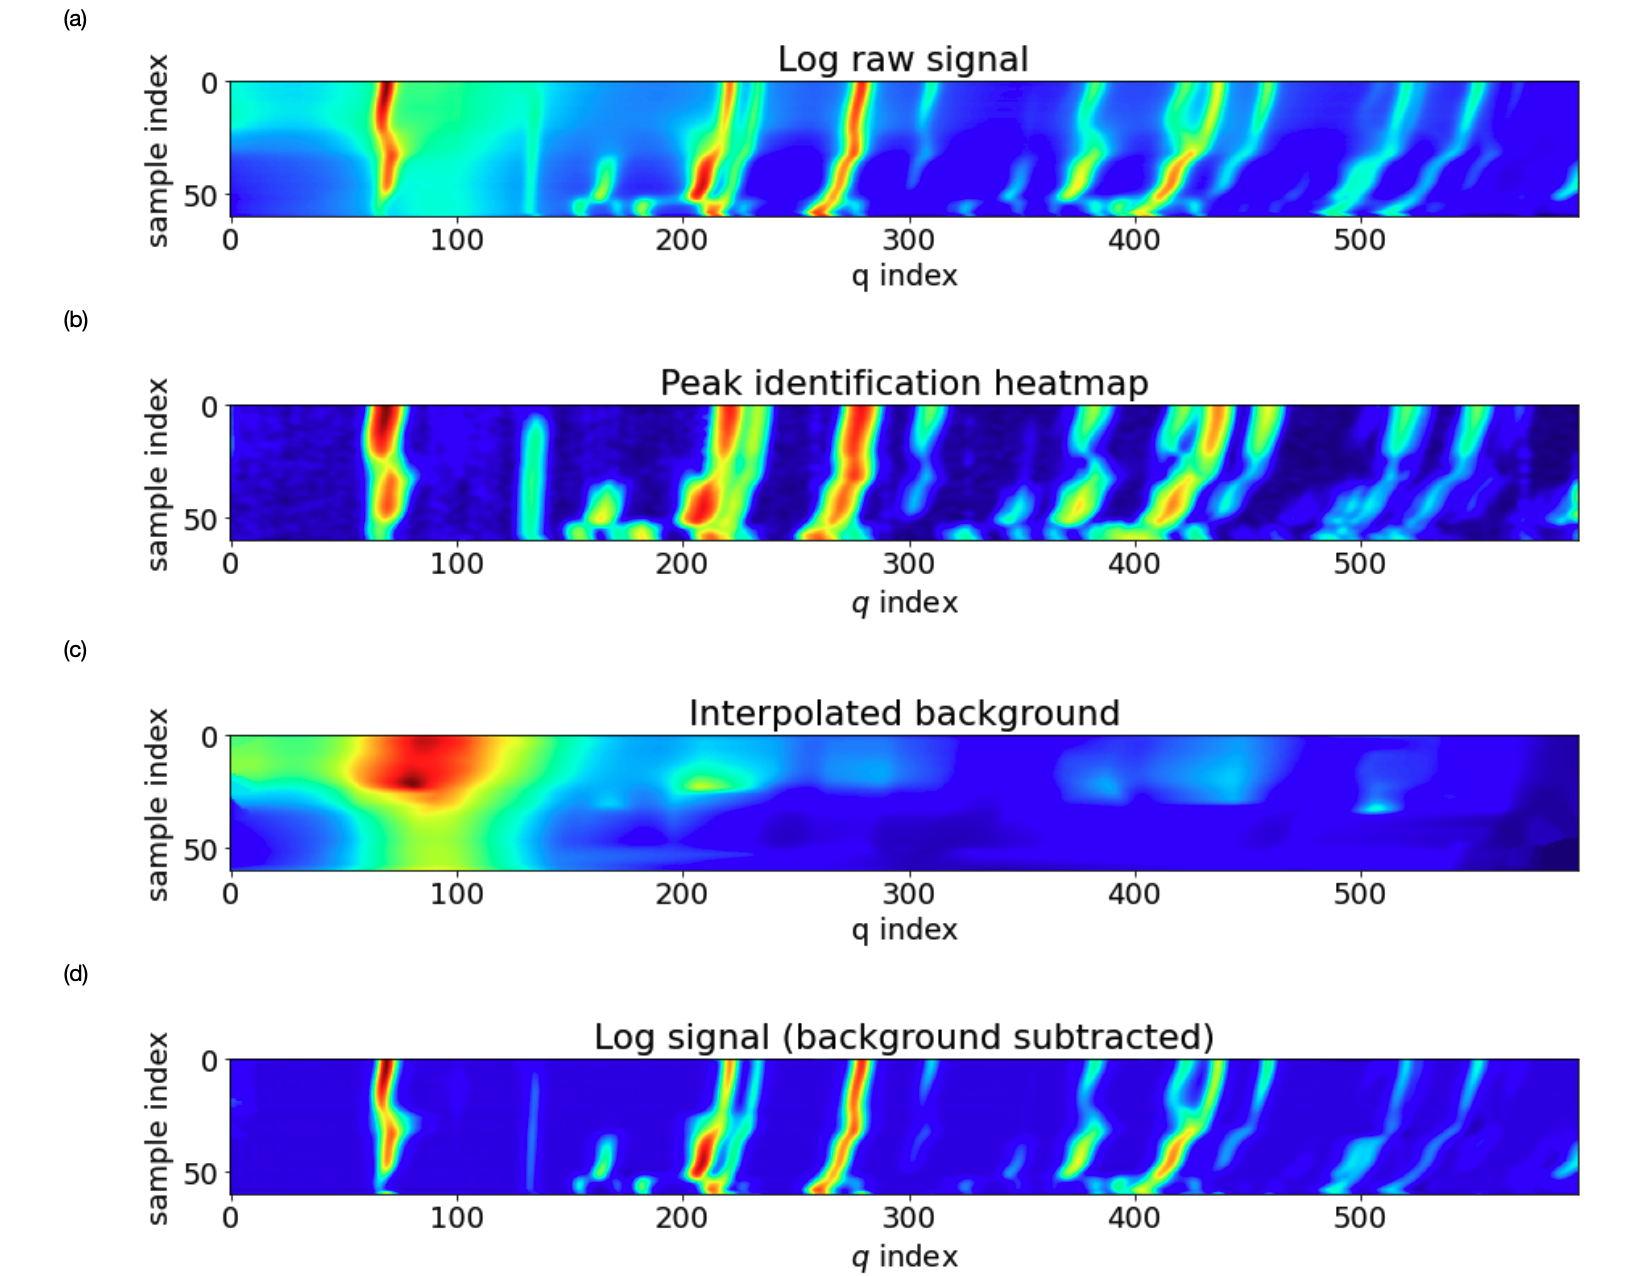
\includegraphics[width=\linewidth]{figures/heatmaps.png}
  \caption{
 (a) Heatmap of XRD dataset $X_{iq}$ corresponding to a temperature scan
of XRD patterns for xxxxx system. The vertical index $i$ and horizontal
index $q$ index temperature and momentum transfer, respectively.

(b) ...

(c)

(d)}
  \label{fig:heatmaps}
\end{figure}
%Separation: either fast/slow or frequency-based variation. Frequency of variation is the key idea. 
%
%Alternative: median / quartile variation based on population density. Acknowledge these alternatives. 
%
%Consider cost of computation: what's the method that would allow an event-detection-type setup. See if we could sell this type of thing to the detector group at SLAC that works on ASICS for rare evetns. 
\subsection{Background subtraction}
The first step to estimating the background is to identify the peak
regions, which must be excluded before calculating the background. In
the case of typical diffraction data a simple high-pass DFT filter does
not cleanly extract the peaks when phase is retained in the inverse
Fourier transform. This is because of the presence of ringing artifacts
as well as the high concentration of signal in the diffraction peaks,
which pile on top of the background in the low-frequency region of the
power spectral density. On the other hand we can identify peak regions
by applying a threshold on the transformed signal illustrated in Fig.
1(b), which we calculate as

\begin{equation}
N(0, \sigma) \circledast |{F}^{-1}(H  {F}(q))|,
\end{equation}

where $N$ is a unit Gaussian in q with standard deviation $\sigma$
is chosen to match the diffraction peak width, $\circledast$ denotes
convolution, and $H$ is a high-pass Gaussian window. The background can
then be simply estimated by an interpolation using data from non-peak
regions to fill in background intensities within the peak regions (Fig.
1(c)) and finally subtracted from the denoised data (Fig. 1(d)).

To make for a simple extension to datasets of arbitrary dimensions we
estimate the background by linear interpolation in the q dimension
alone, together with an N-dimensional nearest-neighbor assignment to
fill in points out of range for interpolation.

\subsection{Noise estimation}
\begin{figure}
  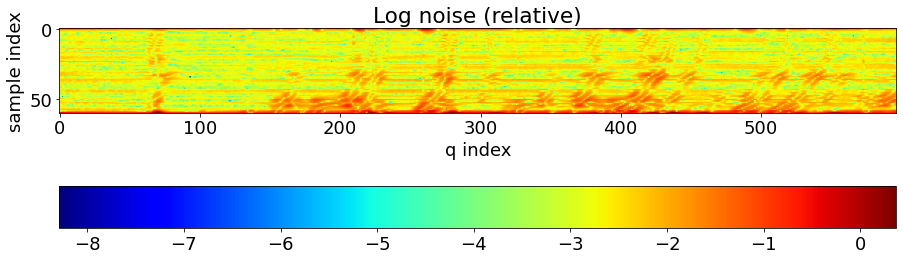
\includegraphics[width=\linewidth]{figures/noise.png}
  \caption{}
  \label{fig:noise}
\end{figure}
While in the case of intensity variation in the q dimension we assume
that high-frequency features belong to the informative (i.e. physical)
component of the signal, in the case of the ordering dimensions we
make the opposite assumption that the physically relevant part of the
signal varies smoothly from one XRD pattern to any adjacent one, while
any high-frequency, uncorrelated deviations from this progression are
due to either noise (from e.g. detector characteristics or Poisson
statistics) or artifacts (such as insufficient orientational sampling
of the diffracting crystallites). Under this assumption the signal and
noise lack substantial overlap in the N-1-dimensional Fourier transform
along ordering dimensions; thus we can use a simple DFT filter to
separate them (Fig. 2)

The above estimations of background and noise components separate
the signal into estimates of the physical components (separated into
background + diffuse scattering and diffraction) and uncertainty values
that correspond to single samples of an underlying noise distributions.
Despite its incompleteness, the latter can be used as an input for
sensitivity analysis on downstream models.

\section{Discussion}
\subsection{Application: feature extraction}
The above analysis addresses the data itself, with no scientific
interpretation aside from the separation between crystalline and diffuse
contributions to the scattering signal. However, we find that the same
ordering and smoothness properties are useful for reducing the data into
salient *information*, where the goal is to find physically-meaningful
boundaries in the ordering dimensions corresponding to, e.g., the
surface separating a single-phase region from surrounding multi-phase
regions in a combinatorial diffraction dataset. Specifically, we can
identify diffraction peaks in every XRD pattern, independently, and then
link each peak in a pattern to any peaks in adjacent patterns centered
at a nearby $q$ value. We next define each set of linked peaks as a
*feature* . ….. utility of this is that it removes peak-shifting,
etc….

\begin{figure}
  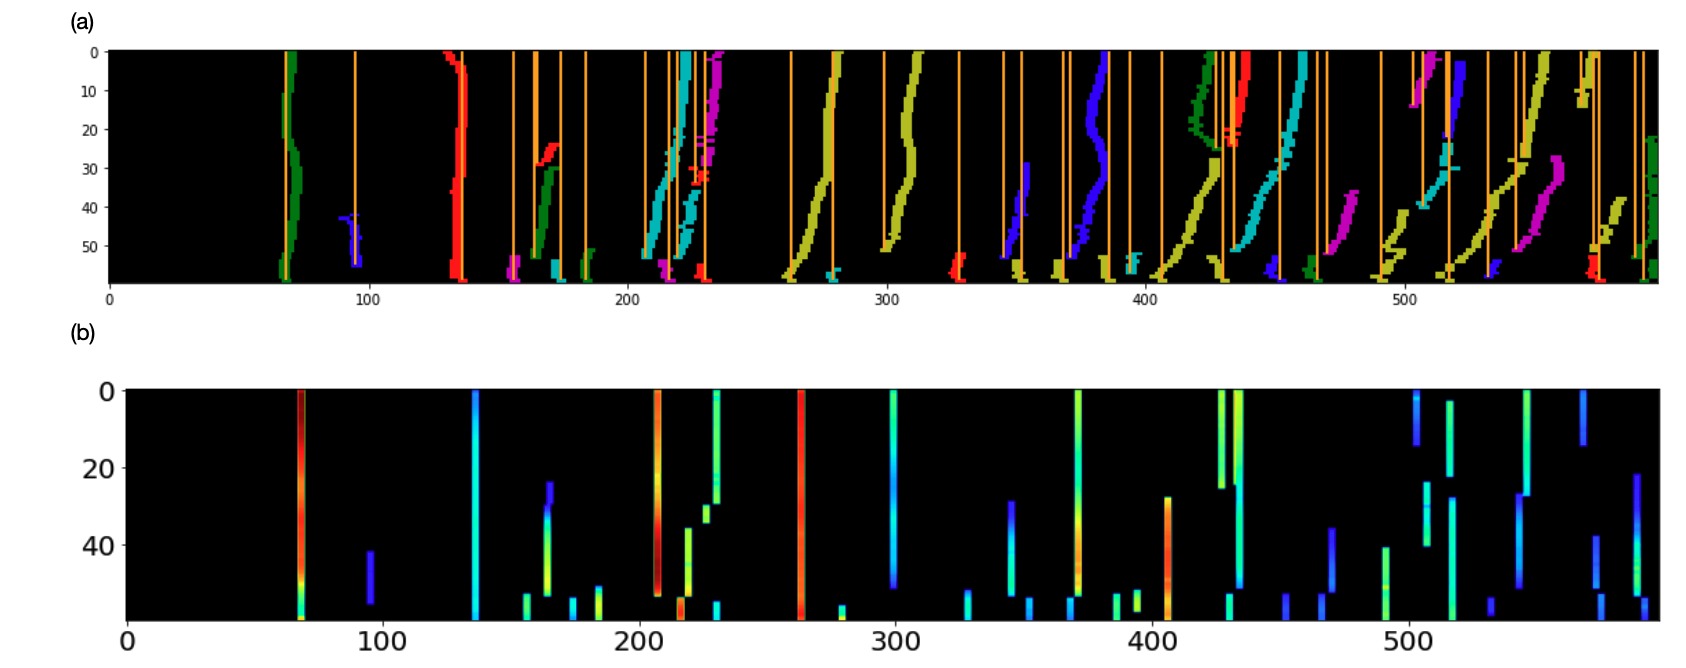
\includegraphics[width=\linewidth]{figures/features.png}
  \caption{(a) Color-coded features identified from peaks connected in
$i,q$ space for XRD dataset $X_{iq}$ corresponding to a temperature scan
of XRD patterns for xxxxxx system. Index $i$ denotes temperature.
    
(b) Intensity profile along each of the features in (a).}
  \label{fig:features}
\end{figure}

%* Discuss caveats: some features are broken up, others are merged. Since there's typically plenty of reduncancy due to the multiple lines that appear with each phase, we think that the feature extraction is robust to these errors.
%* Further interpretation: this is a dimensionality reduction technique. Not a scientific methodology in itself (i.e. the extracted information still has to be interpreted), but a possible improvment over prior methods that are very fragile with respect to peak shifts. 

\section{Conclusions and future work}

\section{References}

\end{document}
